\documentclass[a4paper,9pt,twoside]{article}


\usepackage[utf8]{inputenc}
\usepackage{graphicx}
\usepackage{listings}
\usepackage{xcolor}
\usepackage{amsmath}
\usepackage{indentfirst}								% Indent first paragraphs
\usepackage{float}									% Figure placement with multicol
\usepackage{multicol}
\usepackage{cite}									% Proper citations [1-5]
\usepackage[top=2.5cm,bottom=2.5cm,left=3cm,right=3cm,headsep=5mm,headheight=14pt]{geometry}


\setlength{\skip\footins}{5mm}							% Space between footnotes and text
\setlength{\columnsep}{7mm}								% Column separation

\renewcommand{\abstractname}{\vspace{-\baselineskip}}	% Remove "Abstract" from abstract

% make sections to look like chapters
\usepackage{titlesec}
\titleformat{\section}[block]{\Large\scshape}{\thesection.}{1em}{}

% Title
\title{AN END-TO-END ENCRYPTED PROTOCOL FOR CLOUD STORAGE SOLUTIONS}
\author{Paul Feuvraux \\ pfeuvraux@gmail.com}


\begin{document}
\maketitle

% No page number on 1st page
\thispagestyle{empty}

TO BE REVIEWED

%---------------- ABSTRACT ------------------------%

\begin{abstract}

Current cloud storage solutions don't provide enough details 
about their cryptographic protocols, which leads to wrong assumptions from the users. 
In this paper, we describe how to create a scalable protocol for anyone that would want to 
implement the end-to-end encryption within their cloud storage 
software.

    This paper only describes the cryptographic protocol, 
and does not explain the security measures that are taken for the 
clients, the API, or even the infrastucture. Thus, passwords 
managements, or such issues unrelated to the protocol are not 
described within this paper.
\end{abstract}
%------------ END ABSTRACT --------------------%

%\begin{multicols}{2}

%-------------- INTRO -------------------%
\section{Introduction}
Privacy has always been put at risk, and the Internet was never designed with security in mind. 
The lack of security within the Internet design has made it easier for private companies, goverments, or other 
entities to spy on the people, and threathen the universal right to privacy. 
Even though platforms such as  Dropbox take security measures to prevent unauthorized access to their users' data, 
the lack of end-to-end encryption leaves room for data leaks and data reselling from hackers and the data holders themselves. 
By having end-to-end encryption built-in within the platform, such security vulnerabilities are significantly reduced.

    Current solutions tend to use too many primitives which are often inefficient and insecure. 
There appears to be an absence of end-to-end encrypted cloud storage platforms that are also open source, and thus, transparent. 
Our proposed cryptographic protocol is a mix of heavy security practices, and high-speed methods. We recommend this protocol 
to whoever wants to create an end-to-end cloud storage solution, or implement end-to-end encryption within their 
current software architecture.

    In order to avoid breaking most of the common workflows, we decided to make this protocol compatible with the most common
 use cases. Hence, this protocol allows users to share files through a public link, or with their contacts 
in a secure way. Moreover, this protocol also considers \emph{private realms}, 
so that even companies or any entity will be able to have control over access.

%----------------- END INTRO ----------------%

%--------- PROTOCOL -------------------%


\section{Network Model}

Any communication protocol could be used as long as the code running on the 
client-side is hardly amendable such as compiled programs. Yet, as HTTPS is very common, secure, 
and a lot of libraries in many languages exist, we highly recommend it.

The client and server communicate between each other through HTTPS.
Our HTTPS implementation involves the following components:

\begin{itemize}
\item \textbf{Protocol}: TLSv1.2 only
\item \textbf{Encryption algorithm}: Chacha20-Poly1305 or AES-256-GCM-SHA384
\item \textbf{RSA key size}: 4096 bits
\end{itemize}

\begin{figure}[H]
\centering
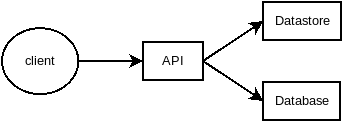
\includegraphics[width=70mm]{./diagram/network_model.png}
\caption{Network Model Overview \label{networkmodel}}
\end{figure}

    As decribed in figure \ref{networkmodel}, the API (the server) is connected to a datastore (hard drive, 
GlusterFS, Ceph, etc.), and a database. All communications are encrypted and an internal Certificate 
Authority is set up in order to limit the MITM attack within the internal network.

    Only the files are stored within the datastore. The files and directories hierarchy is stored within the database 
along with the metadata. For the files and directories hierarchy, JanusGraph is used, for all the other data, 
we use ScyllaDB.

\section{Protocol Functioning}

\subsection{Definitions}

\begin{itemize}
\itemsep0em
\item {Terms}:
\begin{itemize}
\item \textbf{Resource}: defines a file or directory.
\item \textbf{Realm}: defines a space such as an organization, a user's space, etc.
\item \textbf{Encryption Key}: generic name referring to a key used to encrypt a resource.
\item \textbf{$chunk_x$}: refers to any chunk composing a file.
\end{itemize}
\item{Primitives}:
\begin{itemize}
\item \textbf{Library}: Libsodium
\item \textbf{Key Derivation Function}: Argon2-3id
\item \textbf{Encryption Algorithms}: xChacha20-Poly1305 or AES-256-GCM (default)
\item \textbf{Asymmetric Algorithms}: Curve25519 (default) or RSA-4096
\end{itemize}
\item Functions:
\begin{itemize}
\item KDF(P, s): Argon2(P, salt, 7, 65536, 256), where:
\begin{itemize} % start KDF
\item P: Passphrase, can be a UTF-8 string or a binary-formatted key
\item salt: Salt, 128-bit binary array, randomly generated
\item 7: Iterations.
\item 65536: Bytes to be used by the Argon2 function
\item 256: Key size output
\end{itemize} % End KDF
\item Dec/Enc(k, c, n, ad): Encryption / Decryption function
\begin{itemize} %start EncFunc
\item k: 256-bit array (binary formatted)
\item c: un/encrypted content
\item n: Initialization Vector, 128-bit binary array, randomly generated
\item ad: Additional Data: 128-bit binary array, randomly generated
\end{itemize} %end EncFunc
\item rand(size, format): randomly generate data (binary by default). $format$ can be 
binary (0b), hexadecimal (0x), or UTF-8 encoded (utf8).
\item AsymEnc/AsymDec(k, c), where:
\begin{itemize}
\item k: Public or Private Key
\item c: plaintext / ciphertext
\end{itemize}
\end{itemize}
\end{itemize}

\subsection{Key Hierarchy}

\paragraph{}
Users need to share their files and directories in different ways. In order to accomplish this, 
we define a key hierarchy as the following shows:


\begin{itemize}
\itemsep0em
\item \textbf{Content Encryption Key - CEK }: can be considered as a \emph{Root Key}.
\item \textbf{Directory Encryption Key - DEK}: a directory (folder) encryption key, used to derive the 
\emph{FEK} and other \emph{DEK} of a directory's children. Every directory has its own $DEK$.
\item \textbf{File Encryption Key - FEK}: a file encryption key, used to encrypt the data and title 
of files. Each file has got one or multiple $FEK$ depending on its size.
\item \textbf{Parent Encryption Key - PEK}: as defined below, the \emph{Parent Encryption Key} can 
either be the $CEK$ or a $DEK$, depending on the depth. From depth 0, the $PEK$ is 
the $CEK$. For depths $0+n$ (where $n \ge 1$), the $PEK$ will be a $DEK$.
\end{itemize}

\begin{figure}[H]
\centering
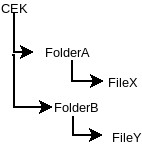
\includegraphics[width=30mm]{./diagram/key_hierarchy.png}
\caption{Key Hierarchy Overview \label{keyhierarchy}}
\end{figure}

    As described in figure \ref{keyhierarchy}, keys are set under a cascaded structure. As a result, 
in order to decrypt fileX, the client would need to decrypt the key of FolderA, 
and $CEK$. This structure allows users to share a whole folder with very few computations.
    The Content Encryption Key can be considered as a \emph{Root Key}. Then, FolderA and Folder B 
have their own keys, derived from the $CEK$. Hence, FileX and FileY have 
their own \emph{File Encryption Keys} respectively derived from FolderA and FolderB keys.

And so, we define three core keys and one relative key:

\subsubsection{Example}
Let's assume that C is a directory within B, and B is a directory within A. Now, we want to move C up to within A, above B. 
We define this procedure such as:

\begin{subequations}
Demonstration:
\begin{align}
    \delta_e=Enc(C, \delta) \\
    C_e=Enc(B, C) \\
    C=Dec(B, C_e) \\
    C_e=Enc(A,C) \\
    C=Dec(A,C_e) \\
    \delta=Dec(C, \delta_e)
\end{align}
\end{subequations}


Where C is the encryption key of the C directory containing files and directories, and 
$\delta$ is the \emph{File Encryption Key} of a file $\delta$ within C directory.

\subsection{Initialization}

    In this section, we describe how the protocol gets initialized during the 
registration procedure.

    During registration, the client generates a \emph{CEK}. Meanwhile, 
the user defines a passphrase \emph{P}. We define two registration procedures:

\begin{itemize}
\itemsep0em
\item Two-Password: user enters a login password and passphrase
\item One-Password: user only enters a login password
\end{itemize}

\subsubsection{Two-Password Method}

During a Two-Password registration, the user defines a \emph{passphrase} named $P$ being a string. In the meantime, the CEK 
is randomly generated over 256 bits. We describe the procedure such as:

\begin{enumerate}
\itemsep0em
\item $CEK=rand(256)$
\item $P=input(keyboard)$
\item $salt=rand(128)$
\item $KEK=KDF(P, salt)$
\item $IV=rand(128), AD=rand(128)$
\item $CEK_e=Enc(KEK, CEK, IV, AD)$
\end{enumerate}

Once $CEK$ is encrypted as in $CEK_e$, the client encapsulates the data such as: 
$packet=(CEK_e||salt||IV||AD)$.

\subsubsection{One-Password Method}

The following method allows the user to type only one password named $PW$. We describe the 
procedure such as:

\begin{enumerate}
\itemsep0em
\item $LoginPassword=input(keyboard)$
\item $salt_l=rand(128)$
\item $LoginPassword=KDF(PW, salt_l)$
\item Client: $SRP(LoginPassword, salt_l)$
\item $CEK=rand(256)$
\item $salt_p=rand(128)$
\item $KEK=KDF(PW, salt_p)$
\item $IV=rand(128), AD=rand(128)$
\item $CEK_e=Enc(KEK, CEK, IV, AD)$
\item $packet=(CEK_e||salt_p||IV||AD)$
\end{enumerate}

Afterwards, $packet$ is sent to the server in order to store it so that 
the user can access their resources from anywhere.

\subsection{Key Decryption}

When a user aims to log in, they're asked their password or passphrase 
depending on 
which password method has been chosen by the user. 
In the case the user has chosen the Two-Password method, this procedure is to be followed:

\begin{enumerate}
\itemsep0em
\item User enters their passphrase $P$
\item Client gets $packet=(CEK_e||salt||IV||AD)$
\item $KEK=KDF(P, salt)$
\item $CEK=Dec(KEK, CEK_e, IV, AD)$
\end{enumerate}

The One-Password method requires more steps, and is described as follows:

\begin{enumerate}
\itemsep0em
\item User enters their password $PW$
\item Client gets $salt_l$
\item $LoginPassword=KDF(PW, salt_l)$
\item Client: $SRP(LoginPassword, salt_l)$ for authentication purposes
\item Once authenticated, Client gets $packet=(CEK_e||salt_p||IV||AD)$ from the server
\item $KEK=KDF(PW, salt_p)$
\item $CEK=Dec(KEK, CEK_e)$ 
\end{enumerate}

Now, the user can encrypt and decrypt their files.

\section{File Handling}

    In this section, we describe in details how the files are encrypted and decrypted, 
and how the titles of files and directories are encrypted and decrypted as well.

\subsection{File Encryption}

To begin with, the title of the file is encrypted as follows:

\begin{enumerate}
\itemsep0em
\item $IV_t=rand(128), AD_t=rand(128)$
\item $salt_1=rand(128)$
\item $FEK_1=KDF(PEK, salt_1)$
\item $title_e=Enc(FEK_1, title, IV_t, AD_t)$
\end{enumerate}

Then, we send the encrypted title for file upload initialization as:

\begin{center}
$packet_t=(title_e, salt_1, IV_t, AD_T)$
\end{center}

Next, the file is split into chunks in order to parallelize the 
encryption and upload. For instance, a file of 600KiB, we
split the file such as:

\begin{center}
\begin{tabular}{ l | c | c }
  \hline
  id & chunk & size (KiB) \\
  0 & $chunk0$ & 512 \\
  1 & $chunk1$ & 88 \\
  \hline
\end{tabular}
\end{center}

    The first chunk will use $FEK_1$ which is used for title encryption 
    right above. By using the same FEK for title encryption and first chunk 
    encryption, we save time during the process. 
    For every next chunk are randomly generated a 128-bit array IV and AD.

\begin{enumerate}
\itemsep0em
\item $salt_x=rand(128)$
\item $FEK=KDF(PEK, salt)$, where $PEK$ is the parent key.
\item $IV=rand(128), AD=rand(128)$
\item $encChunk_x=Enc(FEK_x, chunk_x, IV_x, AD_x)$
\item $title_e=Enc(FEK, title, IV_t, AD_t)$, where $IV_t$ and $AD_t$ are randomly generated.
\end{enumerate}

    PEK meaning \emph{Parent Encryption Key} can either be a DEK or 
can be the CEK in this case of file encryption, depending on the depth of the 
file, as explained above: if the file is at depth-0 (\emph{root}), then the CEK will be used for the key derivation function. 
Otherwise, the DEK of the current directory will be used.


    For every encrypted chunk, the client encapsulates the encrypted content and 
the cryptographic parameters such as:
\begin{center}
$packet_x=(encChunk_x || salt_x || IV_x || AD_x|| IV_t || AD_t)$.
\end{center}

\begin{figure}[H]
\centering
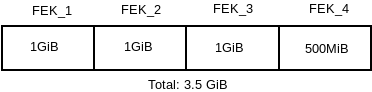
\includegraphics[width=60mm]{./diagram/fek_rotation.png}
\caption{FEK Rotation Overview \label{fekrotation}}
\end{figure}

As figure \ref{fekrotation} describes, once a FEK has encrypted over 1GiB, we proceed to a key rotation by doing 
a key derivation of the parent key of the FEK, as: $FEK_x=KDF(PEK, salt)$, 
where $salt=rand(128)$ and PEK is the parent key of the parent directory. Consequently, a file's size 
between 1GiB and 2GiB will have two File Encryption Keys: $(FEK_1, FEK_2)$, where $FEK_1=FEK$ 
in this section, and so on.

\subsection{File Decryption}

We describe the file decryption procedure as follows:

\begin{enumerate}
\itemsep0em
\item $salt_1$ is obtained from the server for the first File Encryption Key ($FEK_1$) of the file.
\item $FEK_1=KDF(PEK, salt_1)$
\item $chunk_x=Dec(FEK_1, encChunk_x, IV_x, AD_x)$, where $IV_x$ and $AD_x$ are both obtained 
from the server for every chunk.
\end{enumerate}

If the file is larger than 1GiB, then the File Encryption Key will be $FEK_x$, where 
$x$ depends on the count of GiB that has been decrypted.

\subsection{Directory Encryption}

Each directory has its title getting encrypted when being created. We describe 
this procedure as follows:

\begin{enumerate}
\itemsep0em
\item $DEK=KDF(PEK, salt)$, where $salt$ is randomly generated over 128 bits, and 
$DEK$ stands for \emph{Directory Encryption Key}.
\item $IV=rand(128), AD=rand(128)$
\item $dirTitle_e=Enc(DEK, dirTitle, IV, AD)$
\end{enumerate}

Once the title of the directory is encrypted, the client sends a packet to the server, defined as: 

\begin{center}
$packet=(dirTitle_e, salt, IV, AD)$
\end{center}

\subsection{Directory Decryption}

We define the decryption procedure such as:

\begin{enumerate}
\itemsep0em
\item $DEK=KDF(PEK, salt)$, where $salt$ is obtained from the server along with $IV$ and $AD$.
\item $dirTitle=Dec(DEK, dirTitle_e, IV, AD)$
\end{enumerate}

Once decrypted, the title is displayed on the client interface.

\subsection{Sharing}

We define two types of sharing procedures:

\begin{itemize}
\itemsep0em
\item \textbf{External Sharing}: share a file or directory through a public link and secret password.
\item \textbf{Internal Sharing}: share a file between \emph{contacts}
\end{itemize}

External sharing allows a user to share either a file or directory through a public link 
and a defined password. We describe this procedure as:

\begin{enumerate}
\itemsep0em
\item $EK=KDF(PEK, salt_e)$, where $EK$ means \emph{Encryption Key} 
and can either be a FEK or a DEK depending on the type of resource 
to be shared (file / directory), and $salt_e$ is obtained from the server.
\item $DK=KDF(SP, salt_d)$, where $SP$ is the entered secret passphrase for the 
resource to be shared, and $salt_d$ is randomly generated over 128 bits.
\item $EK_e=Enc(DK, EK, IV, AD)$, where $IV$ and $AD$ are randomly generated 
over 128 bits.
\item Client sends $packet=(EK_e || salt_d || IV || AD)$.
\end{enumerate}

    Now, anyone with the generated public link and password can access the resource, such as:

\begin{enumerate}
\itemsep0em
\item Client gets $packet=(EK_e || salt_d || IV || AD)$ from Server.
\item User enters $SP$
\item $DK=KDF(SP, salt_d)$
\item $EK=Dec(DK, EK_e, IV, AD)$
\item $chunk_x=Dec(EK, encChunk_x, IV_x, AD_x)$
\end{enumerate}


Users should be able to share resources between each other in a secure and automated 
way. We introduce the notion of Contacts later. As the Contacts notion is yet not defined, 
we assume that the Public Key of a user's contact 
is safely encrypted and stored by the server. In order to use it, the client needs to get it from 
the server and decrypt it.

    And so, we define the Internal Sharing procedure as follows:

\begin{enumerate}
\itemsep0em
\item Client gets user's contact's Encrypted Public Key ($PKB_e$).
\item $PKB=Dec(CEK, PKB_e, IV, AD)$, where $IV$ and $AD$ are obtained from the server.
\item $EK_e=AsymEnc(PKB, EK)$
\end{enumerate}

    From that point on, the user's contact is now able to decrypt the Encryption Key of the 
resource (file or directory), and access it, such as:

\begin{enumerate}
\itemsep0em
\item Client gets $EK_e$, and we assume that the user's private key $PKA$ has already been decrypted.
\item $EK=Dec(PKA, EK_e)$
\item $chunk_x=Dec(EK, encChunk_x, IV_x, AD_x)$
\end{enumerate}

From that point on, the user's contact will be able to download and decrypt every chunk of the file.

\subsection{Comments on Files \& Directories}

Users are able to comment on files and directories, and react to each other's comments the 
way people react on Slack, Discord, or Facebook. When sharing a resource, the user's client derives the first $FEK$ of the file into 
a \emph{Social Encryption Key - SEK}, which will be used to encrypt comments and 
reactions. We describe this procedure as follows:

\begin{enumerate}
\itemsep0em
\item $salt=rand(128)$
\item $SEK=KDF(FEK_1, salt)$
\item $IV_x=rand(128), AD_x=rand(128)$
\item $encComm_x=Enc(SEK, comm_x, IV_x, AD_x)$
\item $packet=(encComm||salt||IV_x||AD_x)$
\item $send(packet)$
\end{enumerate}

As described right above, an IV and AD are generated over 128 bits 
for every comment. Now, anyone having access to the resource will be able to 
decrypt $FEK_1$, and hence will be able to derive it into the $SEK$ with 
the salt. We describe the procedure such as:

\begin{enumerate}
\itemsep0em
\item Client decrypts $FEK_1$ as explained in the above sections.
\item $SEK=KDF(FEK_1, salt)$
\item $comm_x=Dec(SEK, encComm_x, IV_x, AD_x)$
\end{enumerate}

Multiple comments can be retrieved from the server and decrypted in the meantime 
in order to display them faster on the user interface.

\subsection{Device Syncing}

All user's clients should be able to sync each other without interaction, and 
using the end-to-end encryption in order for users to access their files 
natively from any device through the native file explorer of the operating system.

In order to save bandwidth, devices do not sync between each other by exchanging 
the entirety of the modified files. However, differential deltas will be encrypted 
and then broadcasted to all the devices. Differential deltas will be stored temporary, 
so if a device is out of network for a time range longer than the differential delta 
is supposed to be kept on the servers, the device will need to download the whole 
file once it gets connected back. \textbf{VCDIFF} is the format that we will use in order 
to manage the differential deltas and apply them on the other devices.

\begin{figure}[H]
\centering
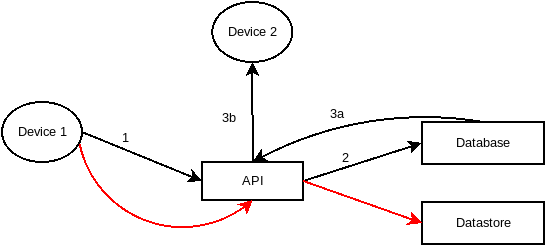
\includegraphics[width=70mm]{./diagram/differentialdeltaarchitecture.png}
\caption{Syncing Model Overview \label{diffdeltaarchi}}
\end{figure}

In red is the whole file being encrypted, uploaded, and then stored within the datastore. 
This ensures that the user will still have access to the file even through the web. Black arrows 
describe the steps of the data differencing system. Device 1 computes the differential delta, 
encrypts it, and sends it to the API server, which will store it within the database, and device 2 
will be able to retrieve the delta later on. However,  if device 2 is connected to the Internet 
and is ready to sync, then the API server will send the differential delta right away in order 
for device 2 to sync it without delay. This system allows our infrastructure to be less used, as 
no READ request is required from the API server in the case device 2 is ready to sync.

\section{Organization Features}

\subsection{Groups and Communities}

\subsubsection{Group - Type 1}

    Group T-1 is just an alias to group the number of actions that a user needs to 
complete in order to share a resource with their contacts. In other terms, group T-1 
is a way for the user to only tick contacts they want to share resources with, without having 
to manually enter each contacts. Consequently, a user creating a group T-1 only needs to 
enter their contacts once. In the future, the user will just need to enter the group they want 
to share resources with.

\subsubsection{Group - Type 2}

    Group T-2 can also be called as \emph{Communities}. A community is a group 
of users allocating their storage to a group as in a community.

    The \emph{Creator} of a community, while creating it, has their client generate 
a \emph{Group Encryption Key - GEK}. Once the $GEK$ generated, it is shared 
with contacts that are to be part of the community. We describe the procedure as follows:

\begin{enumerate}
\itemsep0em
\item $GEK=rand(256)$
\item \emph{Creator's} client encrypts the GEK:
\end{enumerate}
\begin{center}
$(GEK_e=AsymEnc(PKB_x, GEK)) \lor (GEK_e=Enc(KDF(P, salt_p), GEK)))$
\end{center}

,where $PKB_x$ is a key belonging to one of the Creator's contacts, 
and is decrypted as explained in the sections above. $P$ represents the passphrase 
entered by the Creator in the case the Community is to be public.

As $GEK$ is to be encrypted for every user entering the community, either under 
the users' public keys, or under a passphrase, a community remains a safe 
place for users to share resources without compromising their privacy. $GEK$ 
can be considered as the \emph{Root Key} of the community. When a user from within 
the community wants to upload a file, this procedure     is to be applied:

\begin{enumerate}
\itemsep0em
\item $salt=rand(128)$
\item $FEK=KDF(GEK, salt)$
\item $IV=rand(128), AD=rand(128)$
\item $encChunk=Enc(FEK, chunk, IV, AD)$
\item $packet=(encChunk, salt, IV, AD)$
\end{enumerate}

As described right above, once the file is encrypted, it is encapsulated in a packet 
containing the cryptographic parameters allowing the other users to recompute the 
$FEK$ and decrypt the file.

\subsection{Contacts}

Users are able to add contacts in a secure way. As described above, users can share resources 
between each other allowing them to securely share resources without being victim of a 
\emph{Man-In-The-Middle} attack. In order to use the contacts feature, users' clients need to 
generate a pair of asymmetric keys. We define the following procedure as:

\begin{enumerate}
\itemsep0em
\item $(PKA,PKB)=AsymGen(128, 25519)$
\item $DK_a=KDF(CEK, salt_a)$, where $salt$ is randomly generated over 128 bits.
\item Client generates $IV_a$ and $AD_a$, both over 128 bits.
\item $PKA_e=Enc(CEK, PKA, IV_a, AD_a)$
\item $DK_b=KDF(CEK, salt_b)$, where $salt_b$ is randomly generated over 128 bits.
\item Client generates $IV_b$ and $AD_b$ randomly, over 128 bits.
\item $PKB_e=Enc(CEK, PKB, IV_b, AD_b)$
\end{enumerate}

Afterwards, the client encapsulates the cryptographic parameters along with the keys such as: 
\begin{center}
$packet=(PKB||PKB_e||PKA_e||IV_a||AD_a||IV_b||AD_b||salt_a||salt_b)$ 
\end{center}

The client sends $packet$ to the server in order to store it.

When users have their pair of asymmetric keys generated and stored encrypted, 
they can make a contact request with other users. Let's assume Alice adding Bob as a contact,
 we describe the following procedure such as:

\begin{enumerate}
\itemsep0em
\item Alice's client gets $PKB$, being Bob's public key.
\item Alice's client generates $IV$ and $AD$, both randomly over 128 bits.
\item $PKB_e=Enc(CEK, PKB, IV, AD)$, Alice's client encrypts Bob's Public Key.
\end{enumerate}

    Alice now has Bob's Public Key. Consequently, Bob can now accept Alice's request and execute 
the same procedure. Once Bob is done, they both get able to compare the fingerprint of each other's 
Public Key in order to verify whether or not they have been victim of a \emph{MITM} attack. Every time Alice 
and Bob want to share a resource between each other, they need to get each other's encrypted Public Key and 
share the Encryption Key of the resource, such as:

\begin{enumerate}
\itemsep0em
\item Client gets $packet=(PKB_e, salt, IV, AD)$
\item $DK=KDF(CEK, salt)$
\item $PKB=Dec(DK, PKB_e, IV, AD)$
\item $EK_e=AsymEnc(PKB, EK)$
\end{enumerate}

In order for Alice to verify Bob's fingerprint, Bob shows her a QRCode containing the fingerprint. Alice scans 
the QRCode with her phone, while her phone will fetch Bob's $PKB_e$, decrypt it, compute its fingerprint, and 
compare it with the fingerprint from the QRCode. Furthermore, the contact request can be realized through NFC, 
which guarantees that the Public Keys have not been compromised.

\subsection{Private Realms}

    Some users would want to create a \emph{private realm} (an organization), and control users. 
In order to provide such a feature, we define roles, permissions, a key hierarchy, and 
the cryptography behind this feature. We define several types of roles:

\begin{itemize}
\itemsep0em
\item \textbf{Owner}: has full rights on the private realm
\item \textbf{Master}: has full rights but cannot act upon the Owner
\item \textbf{Admin}: can manage members
\item \textbf{Member}: two types of members:
\begin{itemize}
\item Private Member: admins do not have access to the member's keys.
\item Non-Private Member: admins have access to the member's keys
\end{itemize}
\end{itemize}

During the creation of a private realm, the \emph{Owner} 
generates a pair of asymmetric keys, $(PKA_o, PKB_o)$. Those 
will be used for the admins, master, and the owner to decrypt 
the files of non-private members. Their pair of asymmetric keys of 
the private realm are encrypted under the Owner's $CEK$.

\subsubsection{Admins Creation}
To begin with, any admin has to be a private member and must have access
 to the private realm's keys. Consequently, we define the following steps in 
order for the admin to obtain the keys:

\begin{enumerate}
\itemsep0em
\item Master: creates an admin, an invitation link or QRCode is generated.
\item Admin: clicks on the link or scan the QRCode and generates the keys.
\item Admin: $(PKA_a,PKB_a)=AsymGen(128, 25519)$
\item Admin: encrypts $(PKA_a, PKB_a)$ under their $CEK$.
\item $PK_o=(PKA_o, PKB_o)$
\item Master: $PK_e=AsymEnc(PKB_a, PK_o)$
\item Master: $send(PK_e)$ to the server.
\end{enumerate}

\subsubsection{Non-Private Member Creation}

When an admin creates a non-private user, the keys for this user 
are generated by the admin. We describe the procedure as follows:

\begin{enumerate}
\itemsep0em
\item Client gets encrypted $PKB_o$ of the private realm.
\item Client gets admin's PKA and PKB ($PKA_a, PKB_a$) and decrypt them.
\item $PKB_o=AsymDec(PKA_a, encPKB_o)$
\item $CEK_u=Gen(256)$
\item $(PKA_u, PKB_u)=AsymGen(128, 25519)$
\item $CEK_e=AsymEnc(PKB_o, CEK_u)$
\item $PK_u=(PKA_u,PKB_u)$
\item $PK_e=AsymEnc(PKB_o, PK_u)$
\end{enumerate}

Once $CEK_u$ and $PK_u$ being the non-private member's keys are encrypted, and then sent to the server 
in order to be stored along with their cryptographic parameters. In the meantime, 
$CEK_u$ and $PK_u$ are encrypted under a passphrase  with the same procedure as described in section 
\emph{External Sharing}, where the passphrase is to be given to the user through NFC, 
QR code, e-mail, etc.

\subsubsection{Decrypting a non-private member's resource}

    Admins are able to decrypt non-private member's resources, we define 
the procedure such as:

\begin{enumerate}
\itemsep0em
\item Client gets private realm's $PKA_e$ and decrypts it.
\item $DK=KDF(CEK, salt)$, where $salt$ is obtained along with $PKA_e$ from the server.
\item $PKA=Dec(DK, PKA_e, IV, AD)$, where $IV$ and $AD$ are obtained from the server as well.
\item Client gets $encCEK_u$, which is the non-private member's $CEK$
\item $CEK_u=AsymDec(PKA, encCEK_u)$
\item $chunk_x=Dec(CEK_u, encChunk_x, IV_x, AD_x)$
\end{enumerate}

    As described above, Admins are able to decrypt non-private members' resources.

\subsection{Guests}

\emph{Guests} can be created by any normal user. Although, this feature may be blocked by admins 
within an private realm (organization). When a user creates a, several options are proposed for the creator 
to transmit the Guest Account creation page:

\begin{itemize}
\itemsep0em
\item \textbf{QRCode}: Guest User scan the QRCode which will redirect them to 
the Guest Account creation page.
\item \textbf{Link}: Guest User just needs to click on the link in order to be redirected.
\end{itemize}

Now, when the user accesses the Guest Account Creation page, they can choose several 
options, as described below:

\begin{itemize}
\itemsep0em
\item Passphrase: Guest User enters a passphrase. We define the procedure as:
\begin{enumerate}
\item $(PKA, PKB) = AsymGen(128, 25519)$
\item $IV_a=rand(128), AD_a=rand(128)$
\item $DK_a=KDF(passphrase, salt_a)$, where $salt_a$ is randomly generated.
\item $PKA_e=Enc(DK_a, PKA, IV_a, AD_a)$
\item $IV_b=rand(128), AD=rand(128)$
\item $DK_b=KDF(passphrase, salt_b)$, where $salt_b$ is randomly generated.
\item $PKB_e=Enc(DK_b, PKB, IV_b, AD_b)$
\end{enumerate}
\item QRCode: Keys will be stored within the QRCode along with a link for the Guest User 
to access the resources. We define the procedure as:
\begin{enumerate}
\item $(PKA, PKB)=AsymGen(128, 25519)$
\item $DK=rand(256)$
\item As describe above, $PKA,PKB$ are encrypted under $DK$.
\item Once encrypted and stored on the server, $DK$ is 
converted into a QRCode along with the link of the Guest User realm.
\end{enumerate}
\item File: A file is to be saved by the Guest User, we define the following procedure as:
\begin{enumerate}
\item $DK=rand(256)$
\item As describe above, $PKA, PKB$ are generated and encrypted under $DK$.
\item $DK$ is saved into a file.
\item The file is saved by the Guest User, every time they'll want to access their realm, they'll 
just have to select this file in order to decrypt the content they're accessing.
\end{enumerate}
\end{itemize}

Once $PKB$ and $PKA$ encrypted, Client sends the following:

\begin{center}
$packet=(PKB || PKB_e || PKA_e || salt_a || salt_b || IV_a || AD_a || IV_b || AD_b)$
\end{center}

The User encrypts $PKB$, which is the Public Key of the Guest User. We define the procedure as:

\begin{enumerate}
\itemsep0em
\item $salt=rand(128)$
\item $IV=rand(128), AD=rand(128)$
\item $DK=KDF(CEK, salt)$
\item $PKB_e=Enc(DK, PKB, IV, AD)$
\end{enumerate}

Public Key could be spoofed, it is then recommended that both Guest User and User verify each other's fingerprints.

Users can share resources with the Guests they created. We define the sharing 
procedure as:

\begin{enumerate}
\itemsep0em
\item $DK=KDF(CEK, salt)$, where $salt$ is obtained from the server.
\item $PKB=Dec(DK, PKB_e, IV, AD)$
\item $FEK_e=AsymEnc(PKB, FEK)$, where $FEK$ is to be decrypted as described 
in the above sections.
\end{enumerate}

\section{Evaluation}

We evaluate the security and usability of a perfect implementation of this protocol.

\subsection{Architecture Security Evaluation}

The primitives that are used in this protocol are known 
to be the strongest and safest around. Furthermore, 
the $CEK$ is needed for the user in order for them to access 
their files. An adversary cannot access the $CEK$ as it is encrypted 
before even reaching the server. Files, directories, and their titles 
are encrypted, which means that any adversary having successfully 
penetrated a storage server could at most read the \emph{Access Time, 
Creation Time} and \emph{Modification Time} of a file. This could eventually 
be improved over the future releases.

\subsection{Usability Evaluation}

Since the protocol aims to achieve an end-to-end encryption model, some features 
might not be available such as searching the files by names as titles are encrypted. 
Consequently, some workflows may need some modification from the users' part 
for them to exploit the cloud storage software at its fullest.

\subsection{Scalability}

     This protocol is easily scalable, from one user to thousands. However, the contact 
feature makes it hard to scale. Since the owner of a resource has to encrypt the 
\emph{Encryption Key} of the resource for every contact, having many contacts 
to share a resource with will increase the number of computations ($O(n)$, where $n$ 
is the number of contacts to share the document with). However, as Curve25519 is 
the default curve for asymmetric keys and operations, this statement is not likely to be true 
unless a huge number of contacts are involved.

In regards to the implementations, web being a very portable platform, any JavaScript implementation of this protocol 
will be slower than a native implementation due to the single-threading architecture of 
JavaScript. Therefore, this protocol will be slow on non-multithreaded languages. In 
order to counter this issue, we recommend developers to parallelize some parts of the protocol, 
such as the encryption of the chunks that can be performed simultaneously.

\subsection{Attack Vectors}

In this section, we discuss some of the most potential attack vectors that could break 
the protocol.

\subsubsection{Web implementations}

    As for every protocol, the implementation of it plays a big role in the security degree 
that can be achieved. Web can be weak, especially when it comes to a very bad \emph{HTTPS} 
implementation. Hence, a bad HTTPS implementation would most likely lead to an undesired 
change in the JavaScript files during the client-server exchanges, resulting to a security breach 
breaking the entirety of the protocol.

\subsubsection{Fingerprints}

    As described in the Contacts section, it is necessary for users to check each other's 
Public Key fingerprint in order to avoid being victim of a MITM attack. If not checked properly, 
the attacker could decrypt every single file that both parts shared with each other.

\subsubsection{Memory-based Attacks}

    In order to limit attacks based on the memory, we recommend developers to shift all the bits 
to zero from the beginning to the end of the chain composing a private parameter, such as a chunk, 
or a key once the client does not need to use it anymore.

\subsubsection{Brute-force}

     In this section, we describe two types of brute-force vectors:

\begin{itemize}
\itemsep0em
\item Brute-force on entered private strings such as passwords or passphrases.
\item Brute-force on the encrypted content.
\end{itemize}

    As required since we want users to access the resources from anywhere, 
the \emph{salt} is not private so that the keys can be recomputed. Consequently, an attacker proceeding to 
a brute-force solution against a passphrase is likely to be a success if users 
do not define strong passphrases. Although, as this protocol uses Argon2 with 
strong parameters, brute-forcing a passphrase remains difficult. Furthermore, as 
AES-256-GCM and xChacha20-Poly1305 are both considered as the strongest primitives 
for encryption, we consider that any resource as practically undecipherable.

\subsubsection{OOB Communication Channel}

External Sharing involves an Out-of-Band communication channel such as e-mails, 
instant messaging, etc. In order for the users to communicate the secret password of an 
externally shared resource, users should use an end-to-end compliant channel. Otherwise, 
in the case of sending plaintext e-mails or plaintext instant messges, the secret password of the externally shared resoure 
could be intercepted by the provider of this OOB communication channel.

\subsection{Zero-Knowledge Proof}

In order to prove that our system complies with the end-to-end encryption principle, 
we define a procedure to follow in order to run tests against the protocol.

\subsubsection{Key Derivation Test}

We define a passphrase  $P$, and a salt $S$, and a derived key $K$, where 
$K=KDF(P, S)$.

    In order to test the safety of the key derivation process, we generate $P$ and $S$ randomly, 
and iterate 10,000 times (this number can be increased). For every iteration, the generated derived key 
is compared with $K$. At the end of the 10,000 iterations, we enter $P$ and $S$ into the key derivation 
function. In normal circumstances, $K$ should equal the generated derived key of the 10,001 iteration.

\subsubsection{Encryption Test}

We proceed to the same method, but now the parameters are:

\begin{itemize}
\itemsep0em
\item $K$, the encryption key.
\item $IV$, an initialization vector (128 bits).
\item $AD$, some additional data (128 bits).
\end{itemize}

    For 10,000 iterations, a key $K_g$ is generated over 256 bits and is used to try to decrypt 
the encrypted resource. At the 10,001 iteration, we use $K$ instead of $K_g$, which should result 
to a successful decryption.

\subsubsection{Safe Transit Test}

    We monitor the exchange between Client and Server over HTTP without SSL/TLS. Client encrypts 
a file and send the chunks in parallel to Server. Our monitoring system has the right key $K$ and the right 
cryptographic parameters of every chunk of every file being $IV$ and $AD$ since both of those parameters are not private. Client 
encrypts and uploads 10,000 files. At the 10,001 file, our monitor uses $K$ to decrypt a chunk of the last file, 
which should result to a successful decryption. Consequently, this shows that as long as the key $K$ is not leaked, 
the protocol remains safe.

\subsection{Security Improvements}

    It is not necessary for contacts to sign off each other's Public Key's fingerprint. And so, in the case of a 
MITM attack, the protocol could be broken. We could indeed wait for a manual action 
from the user in order for them to sign off a fingerprint. Although, in order for our protocol not to be 
too strict when it comes down to the user experience, we only decided to ask the users to make sure 
they manually verify each other's fingerprint.

\section{Conclusion}

    Our protocol has been proven to be secure and compliant with the principle of 
\emph{End-to-End Encryption}. Even though end-to-end encryption is to be 
respected, the protocol does not break most of the common workflows. This protocol 
uses a lot of heavy computations, especially for the key derivation function that is based 
on Argon2. Consequently, systems with very low memory or a full-javacript implementation may end up running out of 
resources, or slowed down during the process of deriving keys. We recommend to 
tweak the Argon2 parameters in order to adapt the protocol for very resource-limited environments, 
and find a good trade-off between security and speed.

\section{Acknowledgements}

\paragraph{}
Thanks to Hoang Long Nguyen for editorial feedback.

%\end{multicols}

\bibliographystyle{unsrt}%Used BibTeX style is unsrt
\bibliography{sample}

\end{document}
